\chapter{Implementacja serwera LSP}
Dysponując parserem kodu Lua, wystarczy odpowiednio przechodzić generowane przez niego drzewa, w celu odpowiedzi na poszczególne zapytania klienta. Punktem wejścia dla projektu będącego częścią niniejszej pracy jest artykuł \cite{lsp_sample} opisujący utworzenie prostego serwera LSP.

\section{Budowa serwera LSP}
\begin{figure}[H]
\centering
Struktura serwera LSP
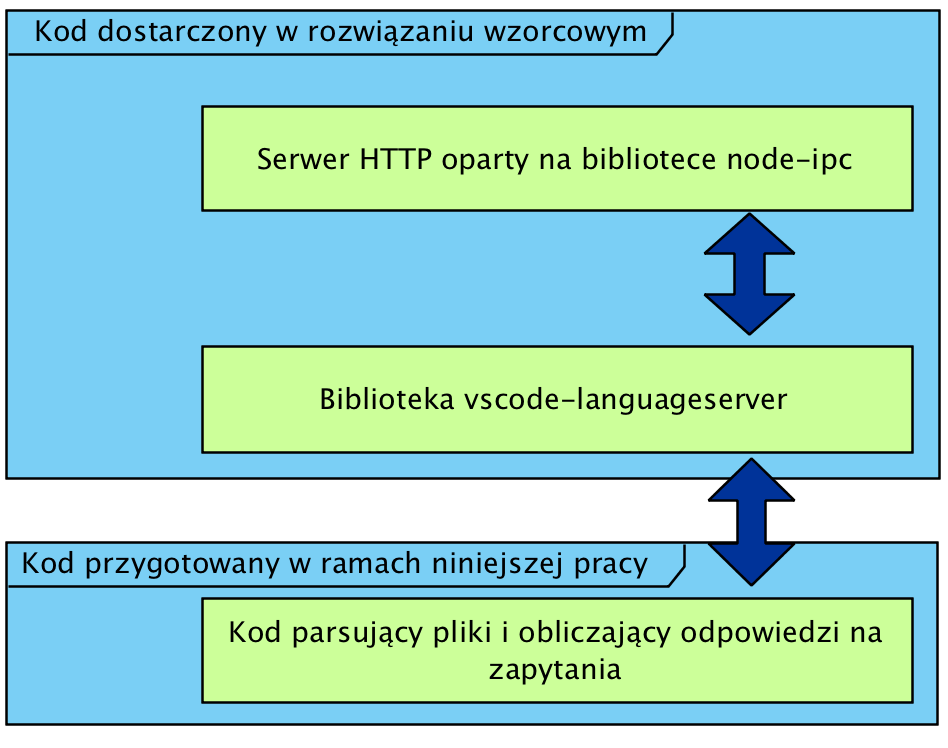
\includegraphics[scale=0.6]{Chapters/struktura_serwera}
\end{figure}

Jak widać na diagramie, kod odpowiedzialny za komunikację w ramach protokołu został dostarczony przez twórców odpowiednich bibliotek. W następnych podrozdziałach poruszana będzie implementacja tej części kodu która oblicza odpowiedzi na zapytania protokołu LSP.

\section{Wypis protokołu LSP}
Protokół LSP, ze względu na szeroką gamę możliwości nowoczesnych edytorów kodu, ma niespełna 40 rodzajów zapytań i komunikatów. Poniżej znajduje się tabela z wypisem metod tegoż interfejsu, a w następnych podrozdziałach nastąpi szczegółowy opis zaimplementowanych w ramach tej pracy rodzajów komunikatów.

\begin{figure}[H]
    \centering
    \small
\begin{tabular}{|c|c|}
\hline
Nazwa metody & Kierunek komunikacji Klient - Serwer\\
\hline
Initialize & $\righttoleftarrow$ \\   
\hline
Initialized & $\rightarrow$ \\
\hline
Shutdown & $\righttoleftarrow$ \\   
\hline
Exit & $\rightarrow$ \\
\hline
ShowMessage & $\leftarrow$ \\
\hline
ShowMessage & $\lefttorightarrow$ \\
\hline
LogMessage & $\leftarrow$ \\
\hline
Telemetry & $\leftarrow$ \\
\hline
RegisterCapability & $\lefttorightarrow$ \\
\hline
UnregisterCapability & $\lefttorightarrow$ \\
\hline
DidChangeConfiguration & $\rightarrow$ \\
\hline
DidChangeWatchedFiles & $\rightarrow$ \\
\hline
Symbol & $\righttoleftarrow$ \\
\hline
ExecuteCommand & $\righttoleftarrow$ \\
\hline
ApplyEdit & $\lefttorightarrow$ \\
\hline
DidOpen & $\rightarrow$ \\
\hline
DidChange & $\rightarrow$ \\
\hline
WillSave & $\rightarrow$ \\
\hline
WillSaveWaitUntil & $\righttoleftarrow$ \\
\hline
DidSave & $\rightarrow$ \\
\hline
DidClose & $\rightarrow$ \\
\hline
PublishDiagnostics & $\leftarrow$ \\
\hline
Completion & $\righttoleftarrow$ \\
\hline
Completion Resolve & $\righttoleftarrow$ \\
\hline
Hover & $\righttoleftarrow$ \\
\hline
SignatureHelp & $\righttoleftarrow$ \\
\hline
Definition & $\righttoleftarrow$ \\
\hline
References & $\righttoleftarrow$ \\
\hline
DocumentHighlight & $\righttoleftarrow$ \\
\hline
DocumentSymbol & $\righttoleftarrow$ \\
\hline
CodeAction & $\righttoleftarrow$ \\
\hline
CodeLens & $\righttoleftarrow$ \\
\hline
CodeLens Resolve & $\righttoleftarrow$ \\
\hline
DocumentLink & $\righttoleftarrow$ \\
\hline
DocumentLink Resolve & $\righttoleftarrow$ \\
\hline
Formatting & $\righttoleftarrow$ \\
\hline
RangeFormatting & $\righttoleftarrow$ \\
\hline
OnTypeFormatting & $\righttoleftarrow$ \\
\hline
Rename & $\righttoleftarrow$ \\
\hline
\end{tabular}
\end{figure}

\section{Zapytanie \texttt{Initialize}}
\begin{lstlisting}[language=JavaScript, basicstyle=\fontsize{9}{10}\ttfamily, title=Struktura argumentu zapytania]
interface InitializeParams {
    processId: number | null
    rootPath?: string | null
    rootUri: DocumentUri | null
    initializationOptions?: any
    capabilities: ClientCapabilities
    trace?: 'off' | 'messages' | 'verbose'
}

interface ClientCapabilities {
    workspace?: WorkspaceClientCapabilities
    textDocument?: TextDocumentClientCapabilities
    experimental?: any
}

interface WorkspaceClientCapabilities {
    applyEdit?: boolean
    workspaceEdit?: { documentChanges?: boolean }
    didChangeConfiguration?: { dynamicRegistration?: boolean }
    didChangeWatchedFiles?: { dynamicRegistration?: boolean }
    symbol?: {
        dynamicRegistration?: boolean
        symbolKind?: { valueSet?: SymbolKind[] }
    }
    executeCommand?: { dynamicRegistration?: boolean }
}

interface TextDocumentClientCapabilities {
    synchronization?: {
        dynamicRegistration?: boolean
        willSave?: boolean
        willSaveWaitUntil?: boolean
        didSave?: boolean
    }
    completion?: {
        dynamicRegistration?: boolean
        completionItem?: {
            snippetSupport?: boolean
            commitCharactersSupport?: boolean
            documentationFormat?: MarkupKind[]
        }
        completionItemKind?: { valueSet?: CompletionItemKind[] }
        contextSupport?: boolean		
    }
    hover?: {
        dynamicRegistration?: boolean
        contentFormat?: MarkupKind[]
    }
    signatureHelp?: {
        dynamicRegistration?: boolean
        signatureInformation?: { documentationFormat?: MarkupKind[] }
    }
    references?: { dynamicRegistration?: boolean }
    documentHighlight?: { dynamicRegistration?: boolean }
    documentSymbol?: {
        dynamicRegistration?: boolean
        symbolKind?: { valueSet?: SymbolKind[] }
    }
    formatting?: { dynamicRegistration?: boolean }
    rangeFormatting?: { dynamicRegistration?: boolean }
    onTypeFormatting?: { dynamicRegistration?: boolean }
    definition?: { dynamicRegistration?: boolean }
    codeAction?: { dynamicRegistration?: boolean }
    codeLens?: { dynamicRegistration?: boolean }
    documentLink?: { dynamicRegistration?: boolean }
	rename?: { dynamicRegistration?: boolean }
}
\end{lstlisting}

\begin{lstlisting}[language=JavaScript, basicstyle=\fontsize{9}{10}\ttfamily, title=Struktura odpowiedzi]
interface InitializeResult {
    capabilities: ServerCapabilities
}

interface ServerCapabilities {
    textDocumentSync?: TextDocumentSyncOptions | number
    hoverProvider?: boolean
    completionProvider?: CompletionOptions
    signatureHelpProvider?: SignatureHelpOptions
    definitionProvider?: boolean
    referencesProvider?: boolean
    documentHighlightProvider?: boolean
    documentSymbolProvider?: boolean
    workspaceSymbolProvider?: boolean
    codeActionProvider?: boolean
    codeLensProvider?: CodeLensOptions
    documentFormattingProvider?: boolean
    documentRangeFormattingProvider?: boolean
    documentOnTypeFormattingProvider?: DocumentOnTypeFormattingOptions
    renameProvider?: boolean
    documentLinkProvider?: DocumentLinkOptions
    executeCommandProvider?: ExecuteCommandOptions
    experimental?: any
}

namespace TextDocumentSyncKind {
     const None = 0
     const Full = 1
     const Incremental = 2
}

interface CompletionOptions {
    resolveProvider?: boolean
    triggerCharacters?: string[]
}

interface SignatureHelpOptions {
    triggerCharacters?: string[]
}

interface CodeLensOptions {
    resolveProvider?: boolean
}

interface DocumentOnTypeFormattingOptions {
    firstTriggerCharacter: string
    moreTriggerCharacter?: string[]
}

interface DocumentLinkOptions {
    resolveProvider?: boolean
}

interface ExecuteCommandOptions {
    commands: string[]
}

interface SaveOptions {
    includeText?: boolean
}

interface TextDocumentSyncOptions {
    openClose?: boolean
    change?: number
    willSave?: boolean
    willSaveWaitUntil?: boolean
    save?: SaveOptions
}
\end{lstlisting}
Zapytanie \texttt{Initialize} posiada masywny interfejs zarówno argumentu zapytania klienta, jak i odpowiedzi serwera. Jest tak ze względu na możliwość implementacji dowolnego fragmentu interfejsu LSP. Przy odpowiadaniu na to zapytanie serwer zwraca przygotowany wcześniej obiekt JSON określający jakie funkcjonalności implementuje. W przypadku tej pracy są to:

\begin{itemize}
    \item Znalezienie definicji danej zmiennej lub funkcji.
    \item Automatyczne sugestie pisanego kodu.
    \item Wyświetlenie informacji na temat danego symbolu.
\end{itemize}

\section{Komunikaty generujące drzewa}
\subsection{Komunikat \texttt{DidChangeTextDocument}}
\begin{lstlisting}[title=Struktura argumentu komunikatu]
interface DidChangeTextDocumentParams {
    textDocument: VersionedTextDocumentIdentifier
    contentChanges: TextDocumentContentChangeEvent[]
}

interface VersionedTextDocumentIdentifier {
    uri: string
    version: number
}

interface TextDocumentContentChangeEvent {
    range?: Range
    rangeLength?: number
    text: string
}

interface Range {
    start: Position
    end: Position
}

interface Position {
    line: number
    character: number
}
\end{lstlisting}

Komunikat \texttt{DidChangeTextDocument} zostaje przesłany do serwera gdy użytkownik zmodyfikował treść pliku (niekoniecznie plik został po tych zmianach zapisany). Należy tutaj nadmienić, że protokół LSP wspiera dwie metody synchronizacji treści pliku między klientem a serwerem, pełną w której każdy komunikat o zmianie pliku zawiera całkowitą treść tego pliku, lub inkrementalny, w którym przesyłane są jedynie pozycje i treść zmienionych fragmentów. Tryb synchronizacji jest określany w odpowiedzi na zapytanie \texttt{Initialize}. Na potrzeby tej pracy zaimplementowano tryb pełny. Po otrzymaniu komunikatu serwer uruchamia parser języka Lua na treści pliku przesłanej w komunikacie. Jeżeli parser napotkał jakiś błąd, jest on zwracany z powrotem do klienta i wyświetlany użytkownikowi pod postacią czerwonego podkreślenia problematycznego fragmentu kodu. Przy udanym parsowaniu otrzymane drzewo jest zapisywane słowniku działającym w roli cache'a, aby można było je odwiedzić przy odpowiadaniu na inne zapytania. Jest to opcjonalna optymalizacja, która pozwala uniknąć ponownego parsowania pliku przy niezmienionej treści. Drzewo dla danego pliku jest ważne tak długo jak nie zostanie dostarczony nowy komunikat świadczący o zmianie treści pliku. Treść pliku również jest zapisywana po stronie serwera za pomocą menadżera otwartych plików dostarczanego przez bibliotekę \texttt{vscode-languageserver}.

\subsection{Komunikat \texttt{DidChangeConfiguration}}
\begin{lstlisting}[title=Struktura argumentu komunikatu]
interface DidChangeConfigurationParams {
    settings: any
}
\end{lstlisting}
Komunikat \texttt{DidChangeConfiguration} informuje nas, że użytkownik zmienił ustawienia edytora, co mogło w różny sposób wpłynąć na proces parsowania otwartych plików. W takim przypadku następuje ponowne parsowanie wszystkich dokumentów znajdujących się w cache serwera, każdy z nich traktując analogicznie do komunikatu \texttt{DidChangeTextDocument}.

\section{Zapytania przechodzące po drzewie}
\subsection{Wizytator \texttt{TraverseTreeDown}}
Każde z zapytań które mają w efekcie przejść się po drzewie rozbioru dostarcza nam informacje na temat pozycji w pliku na której się znajduje kursor. W takim razie wydzielona została funkcjonalność tłumaczenia pozycji na węzeł drzewa. Ponieważ każdy z węzłów drzewa rozbioru zawiera informację na temat zakresu tegoż węzła, wizytator schodzi po drzewie tak długo jak szukana pozycja znajduje się w zakresie przeszukiwanego wierzchołka. Funkcja zwraca wierzchołek na którym zatrzymało się przeszukiwanie.

\subsection{Zapytanie \texttt{Hover}}
\begin{lstlisting}[title=Struktura argumentu zapytania]
interface TextDocumentPositionParams {
    textDocument: string
    position: Position
}
\end{lstlisting}

\begin{lstlisting}[title=Struktura odpowiedzi]
interface Hover {
    contents: MarkedString | MarkedString[]
    range?: Range
}
\end{lstlisting}
Zapytanie \texttt{Hover} zostaje wysłane przez edytor, gdy użytkownik zatrzyma na chwilę kursor myszy nad fragmentem tekstu. Edytor ma wtedy możliwość pokazania dodatkowego okienka zawierającego informacje na temat danego miejsca w kodzie. Serwer w odpowiedzi ma zwrócić treść tegoż okienka, która może być oznakowana za pomocą składni Markdown. Po znalezieniu najlepiej pasującego wierzchołka za pomocą funkcji \texttt{TraverseTreeDown}, zwracany jest tekst którego dokładna treść jest określana na podstawie typu wierzchołka (np. dla funkcji będzie to jej nazwa i lista argumentów, a dla zmiennej jej typ).

\subsection{Zapytanie \texttt{GotoDefinition}}
\begin{lstlisting}[title=Struktura argumentu zapytania]
interface TextDocumentPositionParams {
    textDocument: string
    position: Position
}
\end{lstlisting}

\begin{lstlisting}[title=Struktura odpowiedzi]
type GoToDefinitionReturn = Location | Location[]
\end{lstlisting}
Zapytanie \texttt{GotoDefinition} odpowiada wywołaniu przez użytkownika akcji \textbf{Go to Definition}, polegającej na szukaniu miejsca zdefiniowania w kodzie symbolu znajdującego się pod kursorem myszy. Po znalezieniu szukanego symbolu następuje ponowne przejście po drzewie w celu odnalezienia najpóźniejszej definicji tegoż symbolu (w języku Lua symbole mogą być definiowane na nowo w trakcie działania programu, a także przesłaniane za pomocą słowa kluczowego \texttt{local}). W odpowiedzi zwracana jest pozycja w tekście odnalezionej definicji. Następnie edytor ustawia kursor na otrzymaną pozycję, odkrywając w ten sposób szukaną definicję dla użytkownika.

\subsection{Zapytanie \texttt{Completion}}

\begin{lstlisting}[title=Struktura argumentu zapytania]
interface CompletionParams {
    textDocument: string
    position: Position
    context?: CompletionContext
}

namespace CompletionTriggerKind {
    const Invoked: 1 = 1
    const TriggerCharacter: 2 = 2
}
type CompletionTriggerKind = 1 | 2

interface CompletionContext {
    triggerKind: CompletionTriggerKind
    triggerCharacter?: string
}
\end{lstlisting}
\begin{lstlisting}[title=Struktura odpowiedzi]
interface CompletionList {
    isIncomplete: boolean
    items: CompletionItem[]
}

namespace InsertTextFormat {
    const PlainText = 1
    const Snippet = 2
}

type InsertTextFormat = 1 | 2

interface CompletionItem {
    label: string
    kind?: number
    detail?: string
    documentation?: string | MarkupContent
    sortText?: string
    filterText?: string
    insertText?: string
    insertTextFormat?: InsertTextFormat
    textEdit?: TextEdit
    additionalTextEdits?: TextEdit[]
    commitCharacters?: string[]
    command?: Command
    data?: any
}

namespace CompletionItemKind {
    const Text = 1
    const Method = 2
    const Function = 3
    const Constructor = 4
    const Field = 5
    const Variable = 6
    const Class = 7
    const Interface = 8
    const Module = 9
    const Property = 10
    const Unit = 11
    const Value = 12
    const Enum = 13
    const Keyword = 14
    const Snippet = 15
    const Color = 16
    const File = 17
    const Reference = 18
    const Folder = 19
    const EnumMember = 20
    const Constant = 21
    const Struct = 22
    const Event = 23
    const Operator = 24
    const TypeParameter = 25
}
\end{lstlisting}
Zapytanie \texttt{Completion} jest wysyłane przez klienta w celu odpytania serwera na temat możliwego dokończenia aktualnie pisanego tekstu. Również i w tym przypadku dostarczana jest pozycja kursora, jednakże serwer nie szuka aktualnie edytowanego wierzchołka, tylko listę symboli które zostały zdefiniowane i są dostępne w danym kontekście. Lista odnalezionych symboli jest później rozszerzana o funkcje i zmienne zdefiniowane w bibliotece standardowej Lua (informacje na ich temat znajdują się w osobnym pliku JSON, który został utworzony na podstawie dokumentacji języka \cite{lua_lib}). Obliczona lista zostaje odesłana do klienta, a edytor przed pokazaniem jej użytkownikowi sortuje wpisy pod względem prawdopodobieństwa poprawnego dokończenia wpisywanej frazy.